\documentclass[11pt]{article}
% Defining all packages that are used in this document
\usepackage[utf8]{inputenc}
\usepackage[english]{babel} % Change this to norwegian if report is written in norwegian
\usepackage{amsmath}   % Package for math files
\usepackage{parskip}   % No indent, but instead paragraphs
\usepackage{graphicx}  % Place figures
\usepackage{caption}   % Place captions in tables and figures
\usepackage{subcaption}% 
\usepackage{subfiles}  % 
%\usepackage{subfigure}
\usepackage{pdfpages}
\usepackage[T1]{fontenc} 
\usepackage[euler]{textgreek} % To get greek letters as we know them
\usepackage{amssymb}   % 
\usepackage{placeins}  % \FloatBarrier so figures can't float beyond some point in text
\usepackage{fullpage}  % Uses more of the page
\usepackage{float}     % Able to make figures and tables float \begin{figure}[H] to keep them HERE
\usepackage[version=4]{mhchem} % \ce{} to write chemical eq.
\usepackage{siunitx}   % Ex: \si{\meter\per\square\second}
\usepackage{booktabs}  % Behind-the-scenes optimization of tables. \toprule, \midrule, \bottomrule
\usepackage{multirow}
\usepackage{hyperref}  % Ability to click on references like equations, figures, sections etc. \ref{eq:my_eq} clickable

%表格自动生成
\renewcommand {\thetable} {\thechapter{}.\arabic{table}}
%表格根据章节自动命名
\renewcommand {\thefigure} {\thechapter{}.\arabic{figure}}
%图片根据章节自动命名
\numberwithin{figure}{section}
\numberwithin{table}{section}
\numberwithin{equation}{section}
%以上三个皆控制重命名

\usepackage{fontspec}
\setmainfont{Times New Roman}

\hypersetup{
    colorlinks,
    citecolor=black,
    filecolor=black,
    linkcolor=black,
    urlcolor=black
}
\iffalse
\usepackage{fancyhdr}
	%fancyhdr:一个很强大的宏包,用于自定义设计页面风格并命名以供调用。
	\pagestyle{fancy}
	%\rhead{实验B16 基于vLight的光学仿真基础实验}
	%\lhead{基础物理实验\uppercase\expandafter{\romannumeral2}实验报告}
	\cfoot{ \thepage}  %当前页
	\rfoot{\today}
		%分别是右页眉、左页眉、中页脚、右页脚
	\renewcommand{\headrulewidth}{0pt}
	%\renewcommand{\theenumi}{(\arabic{enumi})}
\fi

\usepackage[autolinebreaks,useliterate,numbered]{mcode} % Ability to paste smooth MATLAB code
\newcommand{\figref}[1]{\figurename~\ref{#1}} %Nice reference to figures
%\linespread{1}
\usepackage{setspace}
\setstretch{1.2}
%\renewcommand{\baselinestretch}{1.5}
\title{
    Robotics design challenge  \\
    (MATLAB/SIMULINK)}
\author{
	Jiaqi, Yao. Ruixin, Zhan. Xuzhao, Zhang. Xiaoyu, Zhang%\footnote{jy431@exeter.ac.uk}
}
%\date{  \today}

\begin{document}
\maketitle
%\begin{abstract}

%\end{abstract}
\pagenumbering{gobble} % Turn off page numbering
%\newpage
%\tableofcontents
%\newpage
\pagenumbering{arabic} % Turn on normal pagenumbering
%%%%%%%%%%%%%%%%%%%%%%%%%%%%%%%%%%%%%%%%%%%%%%%%%%%%%%%%%%
% Main contents - Do NOT write your text in main.tex! Use                     the tex files in the folders below
\section{Brief report}

	\noindent Dear Officer:
	
	\noindent We understand that you are looking for a welding robot for the automotive industry and our team has found our product to be the right fit for your needs. I will then briefly describe our robot and show its advantages in terms of design and precision.
	
	\noindent We have designed a four-armed robot according to your requirements and have considered its parameters, which you can see in Table 1 and Table 2. After simulation analysis, this design is reasonable and can perform the task accurately in the working area. We have also created a kinematic diagram (Figure 2.1) and a workspace diagram (Figure 3.1)
	
	\noindent The maximum error in end effector position on the x and z axes is below 0.05, while the maximum error on the y axis is slightly This shows the amazing accuracy of the robot in its movements and workings. You can see the specific images of the errors in Figure 1 and Figure 2.

\section{Introduction}
\FloatBarrier % Now figures cannot float above section title

Our product is a type of mechanical equipment used for automated welding. Our robotic arm can be widely used in various welding operations in the manufacturing industry, including automotive manufacturing, aerospace, construction, and manufacturing.

Our product has many adavantages. Firstly, it can improve production efficiency and quality by reducing the negative impact of human factors on production through automated welding operations. Secondly, it can reduce the danger of the work environment. 

In summary, the four-arm welding robot is an efficient and accurate welding device with many advantages. It will become an important part of automated production in the manufacturing industry, providing a reliable solution for various production operations.









\iffalse
The purpose of this experiment is to investigate the behaviour of a mild steel portal frame model when subjected to increasing loads.

The rig consists of a loading system that applies a vertical load at the center of the beam and a horizontal load at the top of one column. As shown in \autoref{f0}.

\begin{figure}[htbp]
    \centering
    \includegraphics[width=7.5cm]{./fig/00.jpg}
    \caption{Experimental procedure}
    \label{f0}
\end{figure}

\fi



\section{Task 1}
\FloatBarrier % Now figures cannot float above section title


\subsection{Originality and uniqueness of the robot}

Our robot's uniqueness lies in the fact that it is a four-arm robot. Although two-arm and three-arm robots can perform the same tasks, they are relatively unstable and more difficult to control. In addition, a four-arm robot can provide a larger workspace and a greater potential for improvement.

\subsection{Property of all the arms and the joints}

We have designed 4 joints for the robot, 2 of which are revolute type and 2 are prismatic type. At the same time, there are four corresponding robotic arms, whose parameters are shown in the Table \ref{T 2.1} and Table \ref{T 2.2}.

Furthermore, in order to make the robot operate more stably, we assumed the relevant data of the robot arms, and after simulation, the data we obtained is reasonable.

\begin{minipage}[htbp]{\textwidth}
    \makeatletter\def\@captype{table}
    \centering
    \scalebox{0.9}{
    \begin{tabular}{cccc}
    \hline
    Name & Body Mass (kg) & Center of mass & Inertia ($I_{xx}$ $I_{yy}$ $I_{zz}$) ($kg \cdot m^2$)                  \\ \hline
    R1   & 10        & (0 0 0)        & (0.27 0.27 0.8 )     \\
    R2   & 10        & (0 0 0)        & (0.27 0.27 0.8 )     \\
    P1   & 1.5       & (0 0 0)        & (0.07 0.07 0.07 )    \\
    P2   & 1.5       & (0 0 0)        & (0.07 0.07 0.07 )    \\
    Tool & 1.2       & (0 0 0)        & (0.002 0.002 0.004 ) \\ \hline
    \end{tabular}} 
    \caption{Robot arm parameters}
    \label{T 2.1} 
\end{minipage}


\begin{minipage}[htbp]{\textwidth}
    \makeatletter\def\@captype{table}
    \centering
    \scalebox{1}{
    \begin{tabular}{cccc}
    \hline
    Joint & Type & Position Limit (rad \& m) & Joint Axis                   \\ \hline
    1   & revolute       & $[-5\frac{\pi}{180}, 5\frac{\pi}{180}]$ & [0 0 1]     \\
    2   & revolute       & $[-30\frac{\pi}{180}, 30\frac{\pi}{180}]$        & [0 1 0]     \\
    3   & prismatic      & $[-0.5,0.5]$        & [1 0 0]    \\
    4   & prismatic      & $[-1, 1]$        & [0 1 0]    \\ 
    Fixed &revolute & N/A & N/A \\\hline
    \end{tabular}} 
    \caption{Joint parameters}
    \label{T 2.2} 
\end{minipage}

Figure \ref{F 2.1} is a schematic diagram of the robot in MATLAB.
\begin{figure}[htbp]
    \centering
    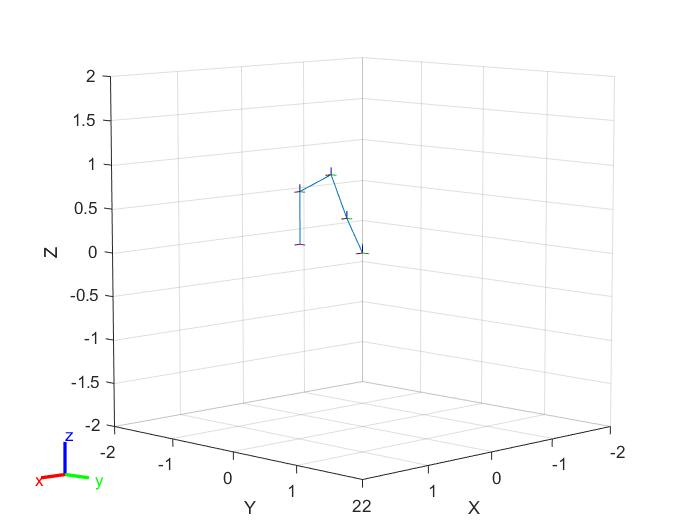
\includegraphics[width=7cm]{./fig/1.jpg}
    \caption{Robot schematic}
    \label{F 2.1}
\end{figure}

\subsection{Collision discussion}

Our designed robot is free from collisions. In most cases, collisions occur on the two arms of the rotating joints whose rotation angle is greater than $±90^\circ$. For our designed robot, the total range of motion for the two movable joints is $±35^\circ$, so there is no collision. Additionally, the animation of the robot's movement trajectory can be viewed in the dynamic image in Figure 8 (After running the matlab code).

\section{Task 2: The Workspace}
\FloatBarrier % Now figures cannot float above section title

Figure \ref{F 3.1} shows the robot's workspace in Task 1. The robot can work with precision within this workspace and also carry out certain tasks outside the range.


\begin{figure}[htbp]
    \centering
    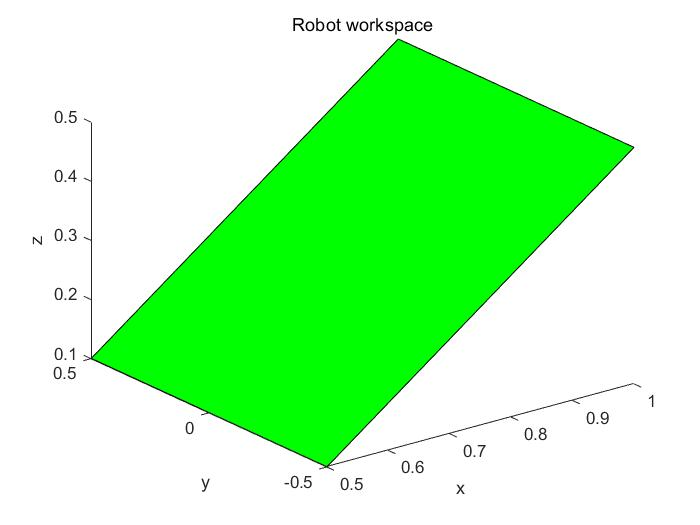
\includegraphics[width=8cm]{./fig/workspace.jpg}
    \caption{Robot's Workspace}
    \label{F 3.1}
\end{figure}






\section{Task 3: The robot's kinematic diagram}
\FloatBarrier % Now figures cannot float above section title

As we can see in the \autoref{F 4.1}, we can find that all the z-axis are the revolution or direction of every joints, and use the right-hand rule, we can check if all the x-axis are perpendicular both to its own z axis and the z axis of the frame before it. Apparently, the directions of all the axis are strictly following the Devenit-Hartenburg Framerules.

\begin{figure}[htbp]
    \centering
    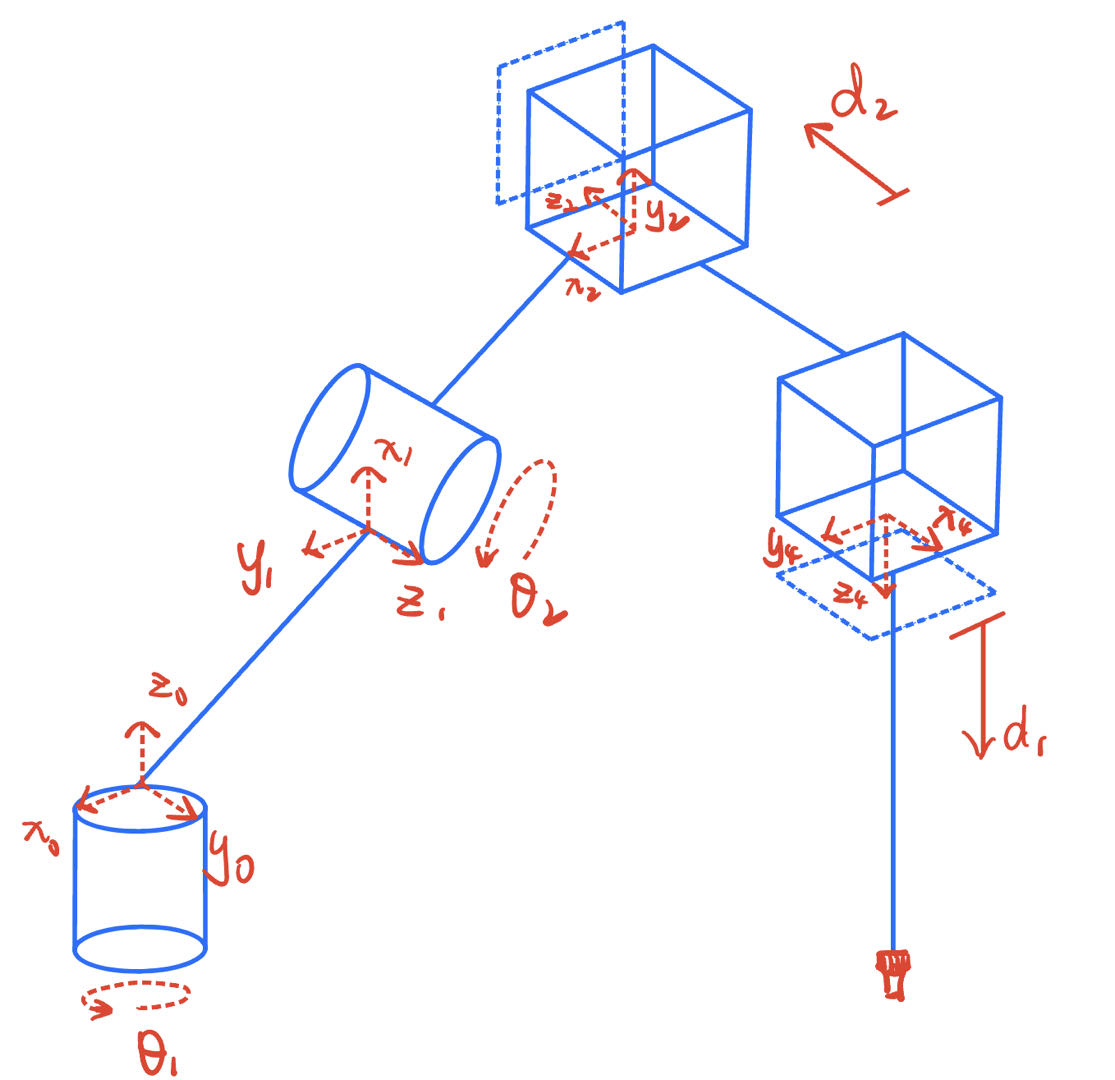
\includegraphics[width=7cm]{./fig/D-H.jpg}
    \caption{The robot's kinematic diagram}
    \label{F 4.1}
\end{figure}

\section{Task 4: Simulink and Simulation}
\FloatBarrier % Now figures cannot float above section title

\subsection{Simulink}
Figure \ref{F 5.1} shows a schematic of Simulink.
\begin{figure}[htp]
    \centering
    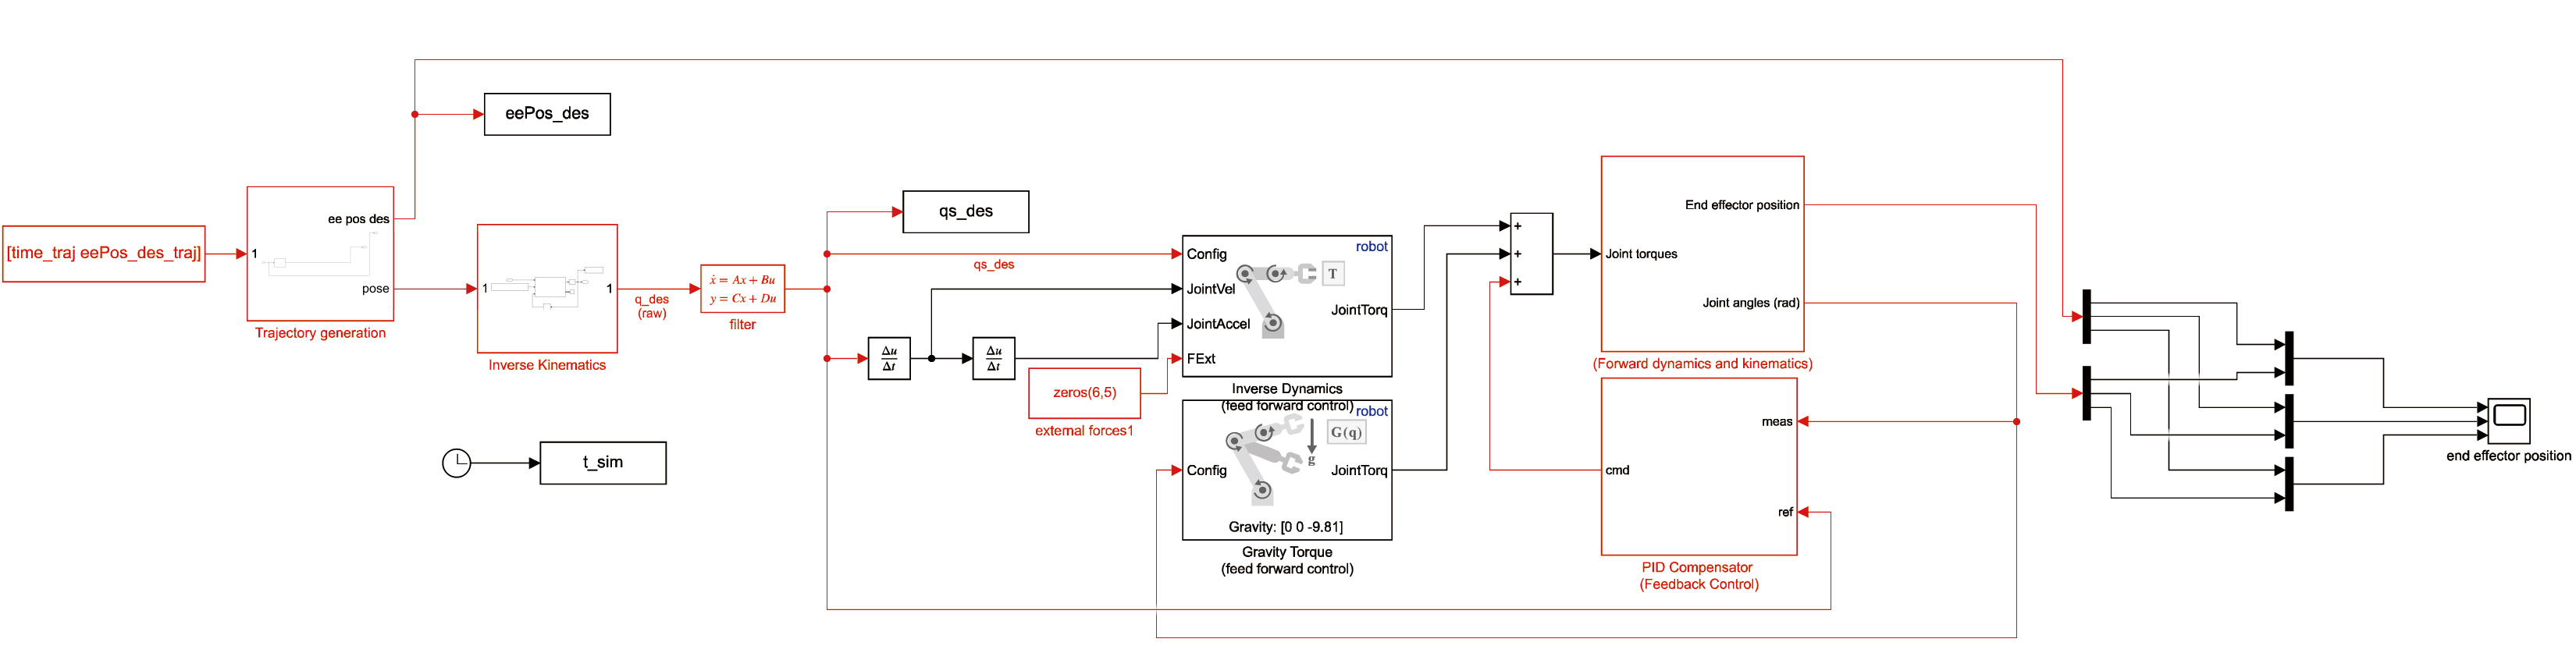
\includegraphics[width=17cm]{./fig/sim.jpg}
    \caption{The Simulink}
    \label{F 5.1}
\end{figure}

\subsubsection*{Tidy of the model}
To ensure aesthetic appeal, a modular design approach was adopted, where different modules represent different functionalities, thereby making the overall model's operation flow appear clear and concise.

\subsubsection*{Trajectory generation}

\begin{figure}[htp]
    \centering
    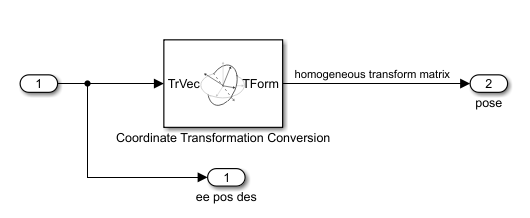
\includegraphics[width=10cm]{./fig/traj.png}
    \caption{Trajectory generation schematic}
    \label{F 5.2}
\end{figure}

We first calculate the path coordinate points and time series from the code, and use them as input parameters for trajectory calculation. Through trajectory calculation as shown in \autoref{F 5.2}, we can obtain the expected end-effector position and obtain motion trajectory data applicable to each point after coordinate transformation (which records the three-dimensional coordinate points of the path every 0.01 seconds).

\begin{figure}[htbp]
	\centering
	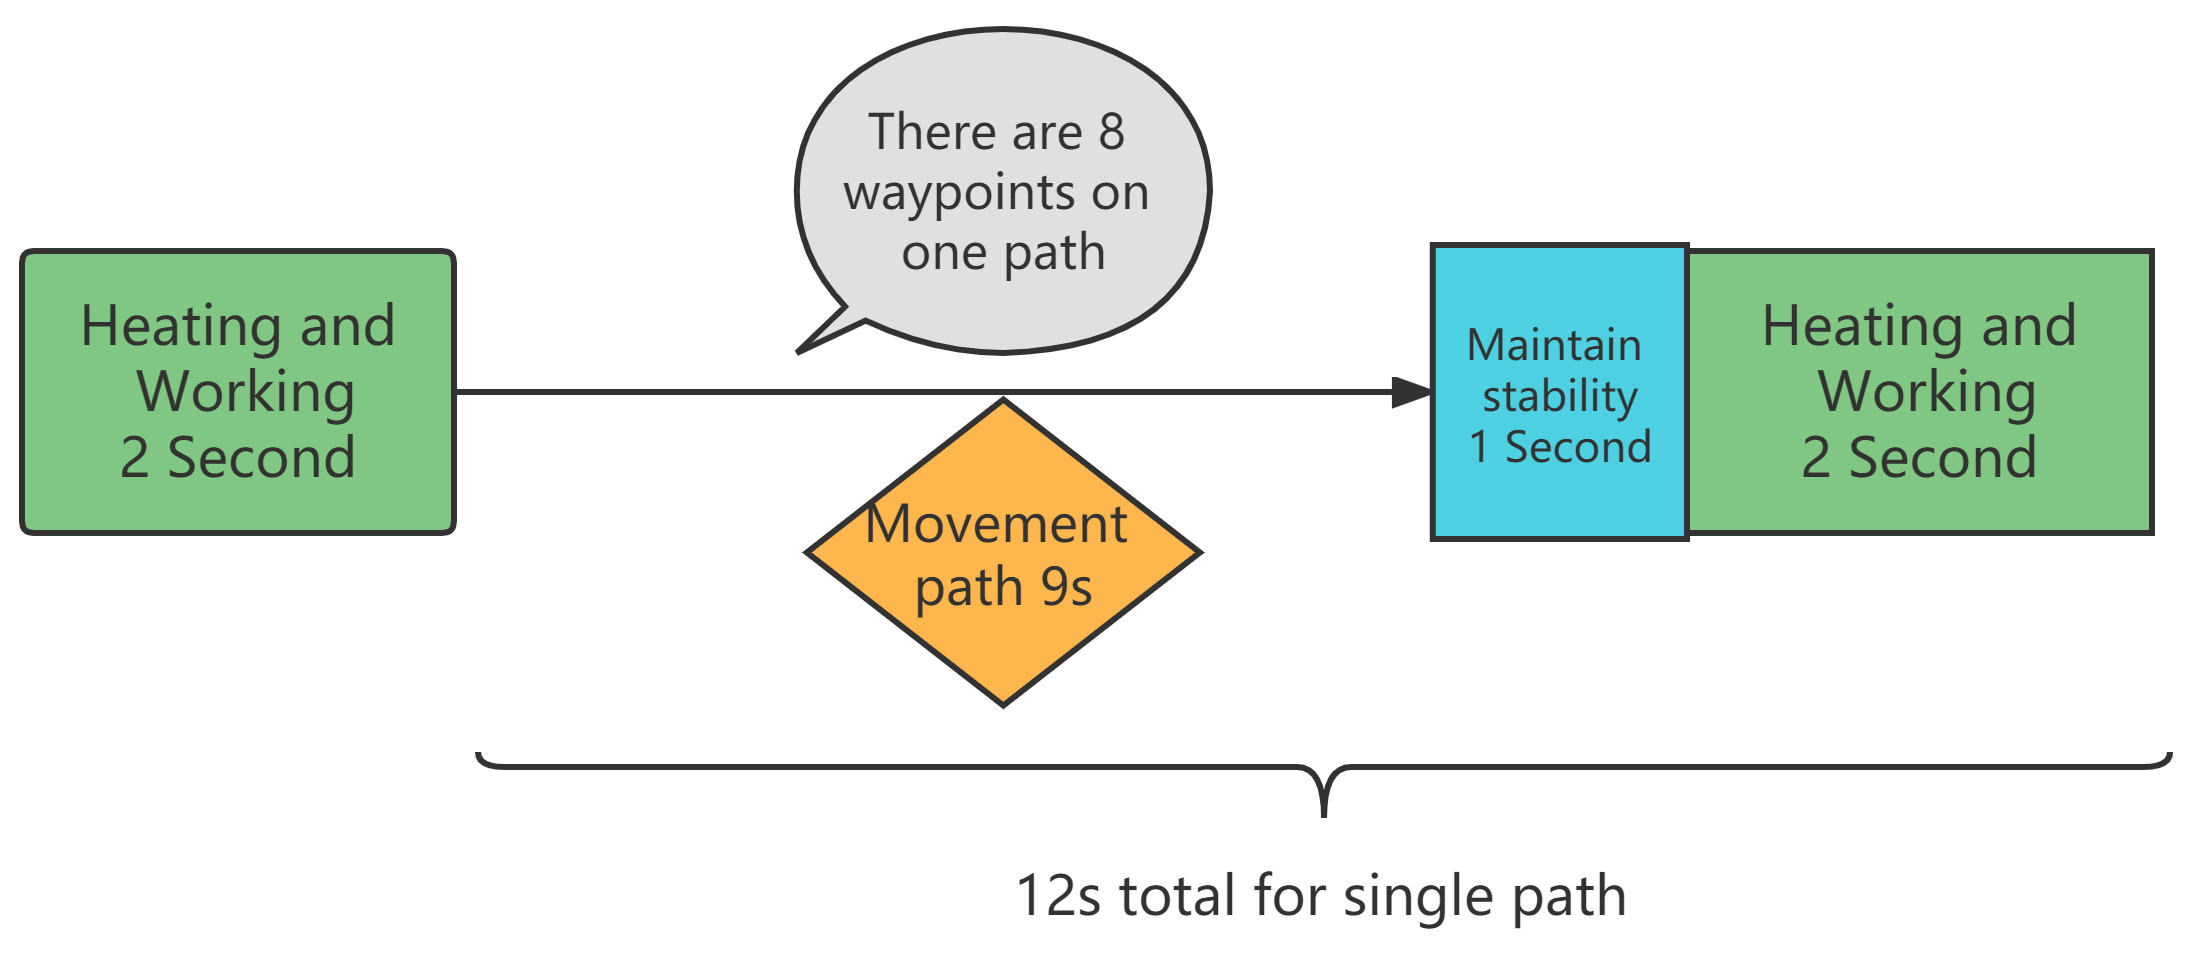
\includegraphics[width=10cm]{./fig/siwei.png}
	\caption{Flowcgart of trajectory generation }
	\label{F 5.3}
\end{figure}

\autoref{F 5.3} is a flowchart of the process we use to compute the trajectory of the robot's end effector position. First, we divide the rectangle required for the task into four line segments. For each line segment, we divide it into 9 equally long segments, and expect the robot to take 9 seconds to move along it. After that, the robot needs to spend 1 second for stabilization, followed by 2 seconds of welding work at the work point. Totally, it takes 48 seconds for the robot to complete the welding task. To account for this, we designed a simulation time of 48 seconds. 

\subsubsection*{Inverse kinematics}

In the inverse kinematics module, we use the expected end-effector position as input, as shown in \autoref{F 5.4}, and calculate the expected joint angles using inverse kinematics. The output is a matrix containing time-series data, which records the rotation angles of different joints of the robotic arm every 0.01 seconds.
\begin{figure}[htbp]
	\centering
	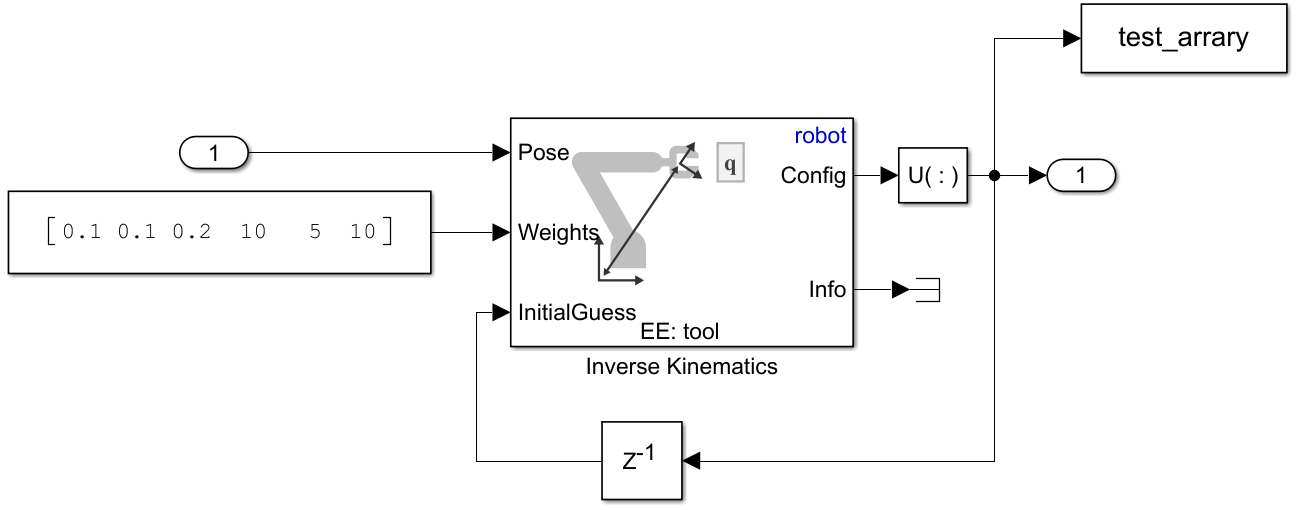
\includegraphics[width=8cm]{./fig/IK.png}
	\caption{Inverse kinematics}
	\label{F 5.4}
\end{figure}

\subsubsection*{Inverse dynamics}

Inverse dynamics is to calculate the forces or torques that are required to produce a desired motion of a robotic system. The technique involves using the system's equations of motion to determine the forces or torques required to generate a desired trajectory or motion. As shown in \autoref{F 5.5}, the input parameter in this part is the coordinate data of each sampling point calculated by the inverse kinematics. By weighting and differentiating the data, the required angular velocity and angular acceleration can be obtained. Then, the obtained data is imported into the inverse dynamics module for calculation, and the result is the torque required for each joint at each sampling point.

\begin{figure}[htbp]
	\centering
	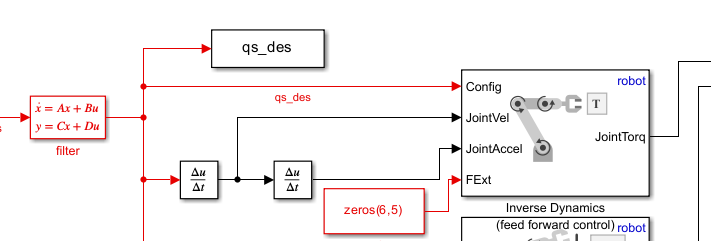
\includegraphics[width=10cm]{./fig/ID.png}
	\caption{Inverse dynamics}
	\label{F 5.5}
\end{figure}

\subsubsection*{Gravity}


In this part, the torque generated by gravity is added as a vector to the torque required by each joint calculated by the inverse dynamics module, and the combined torque vector is passed to the next module to simulate the deviation that may occur in the actual robot arm. The process is shown in \autoref{F 5.6}.


\begin{figure}[htbp]
	\centering
	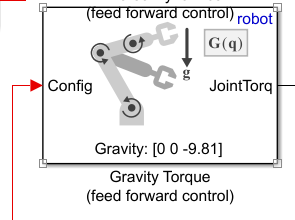
\includegraphics[width=5cm]{./fig/G.png}
	\caption{Gravity part}
	\label{F 5.6}
\end{figure}


\subsubsection*{Forward dynamics and kinematics}


\autoref{F 5.7} shows the forward kinematics and dynamics module, in which the actual position and orientation of the end-effector can be calculated based on the actual joint angles obtained by considering the different torques inputted to each joint.

\begin{figure}[htbp]
	\centering
	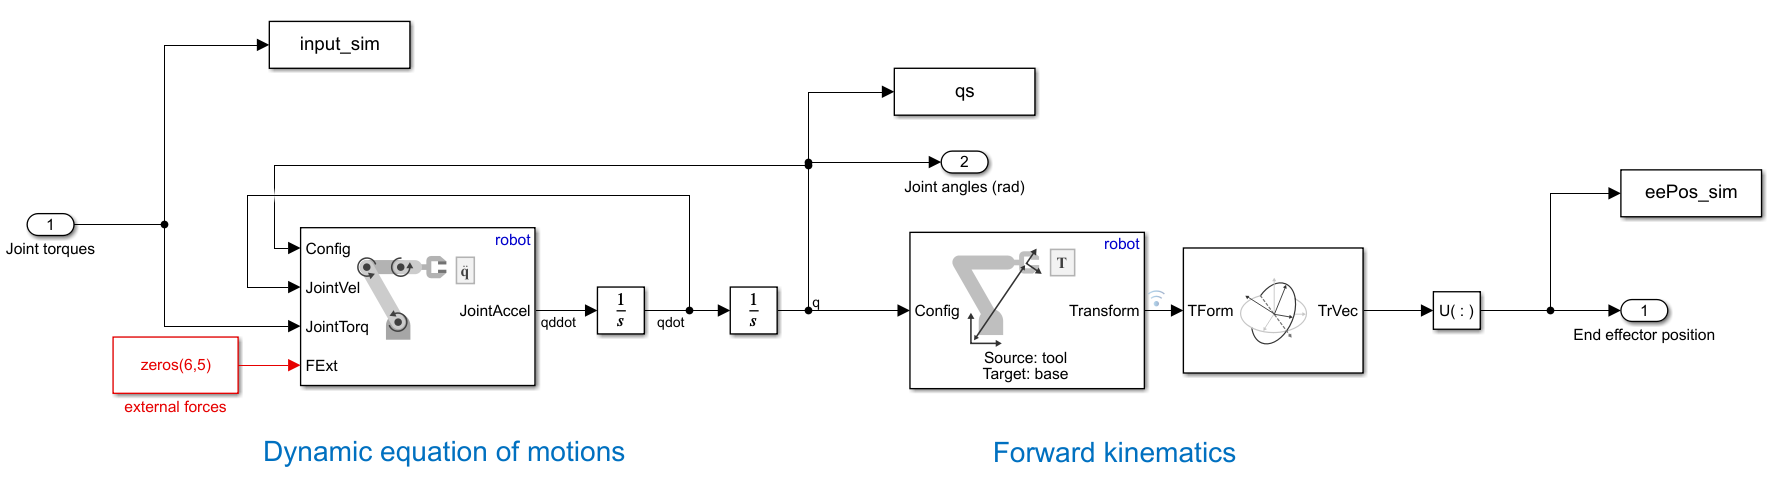
\includegraphics[width=8cm]{./fig/FDK.png}
	\caption{Forward dynamics and kinematics}
	\label{F 5.7}
\end{figure}


\subsection{PID design}



\begin{figure}[htbp]
	\centering
	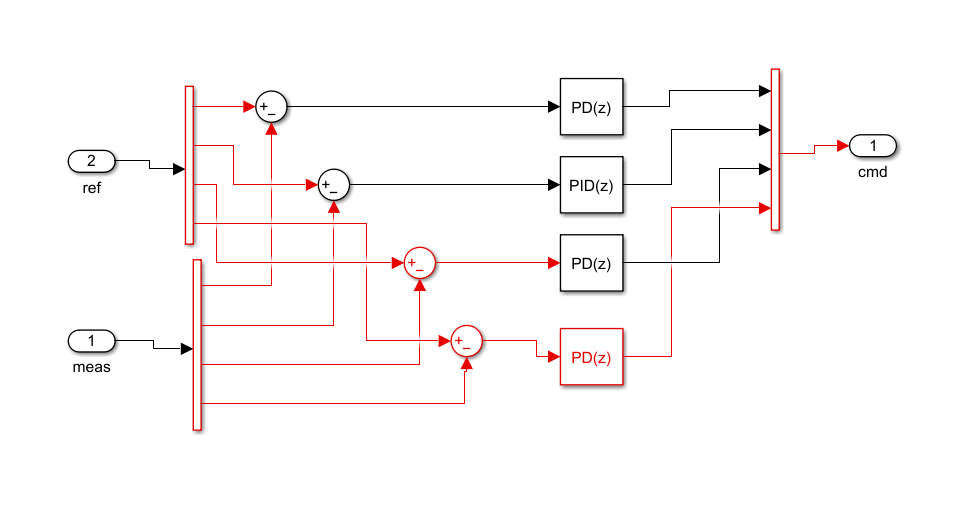
\includegraphics[width=10cm]{./fig/PID.png}
	\caption{PID part}
	\label{F 5.8}
\end{figure}

In the PID control module,as shown in \autoref{F 5.8}, we subtract the desired data from the actual data to obtain the error value, which is then used for PID calculation. We noticed that joints 1, 3, and 4 only use PD controllers because these three joints require a fast response speed and low overshoot, and have lower requirements for steady-state error. For joint 2, which uses a PID controller, it is sensitive to steady-state error due to its rotation around the y-axis. Although there may be difficulty in tuning, we successfully completed the debugging process.


\subsection{Results}

Finally, as shown in \autoref{F 5.9} set the end effector positions and the desired end effector positoins as the input, draw the plot with their x y z positions followed by the time respectively.

\begin{figure}[htbp]
	\centering
	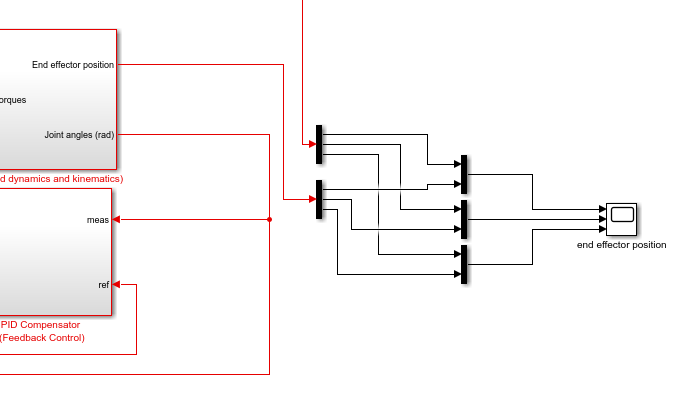
\includegraphics[width=7cm]{./fig/re.png}
	\caption{Export figure part}
	\label{F 5.9}
\end{figure}


\subsubsection*{Input torque}


As shown in \autoref{F 5.10}, this is the torque figure of each joint required for the robot during operation. By observing the figure, it can be found that, except for the initial instability during startup, we only need less than $30N\cdot m$ of torque to drive the robot to complete the welding task.

\begin{figure}[htbp]
	\centering
	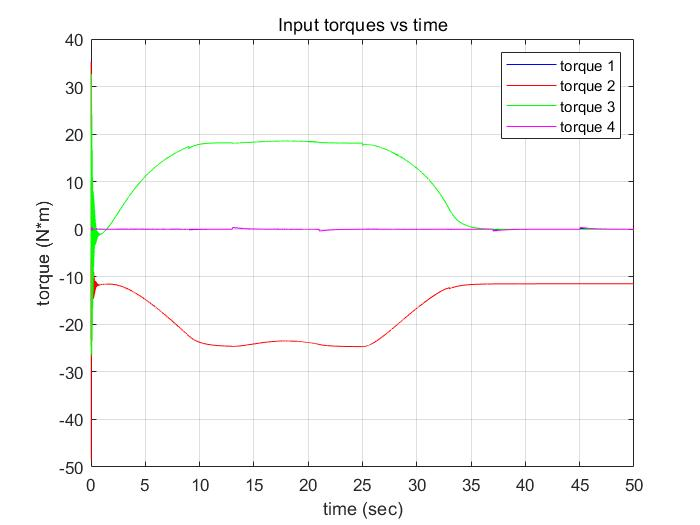
\includegraphics[width=10cm]{./fig/3.jpg}
	\caption{Torque vs Time}
	\label{F 5.10}
\end{figure}

\subsubsection*{Joint angle}




\begin{figure}[htbp]
	\centering
	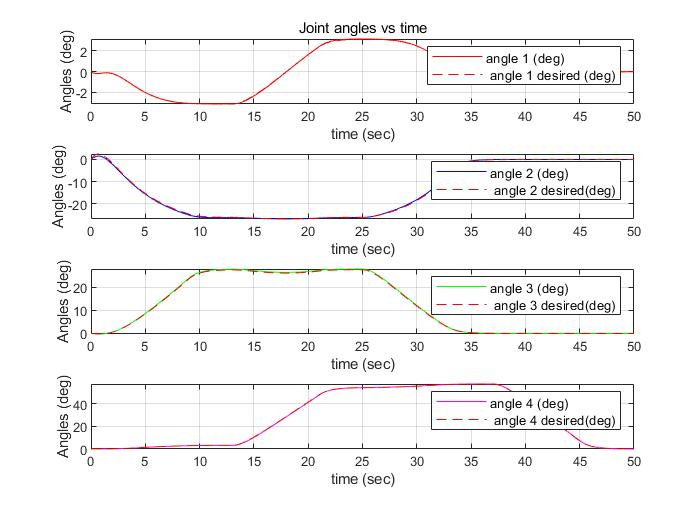
\includegraphics[width=8cm]{./fig/4.jpg}
	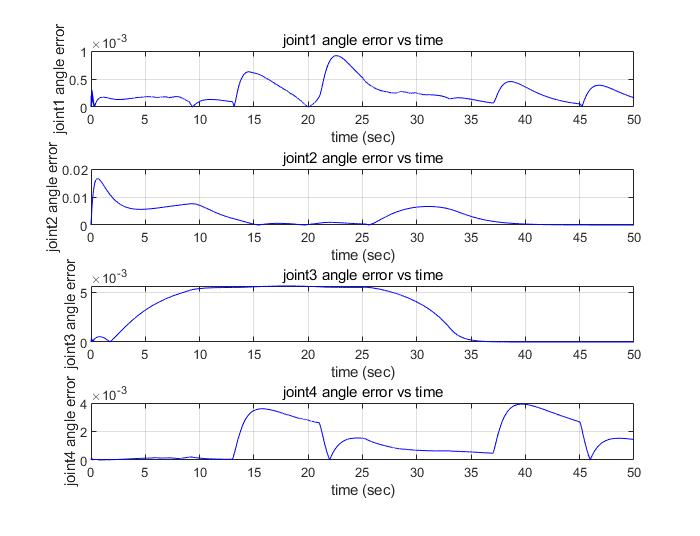
\includegraphics[width=8cm]{./fig/7.jpg}
	\caption{Joint angles vs Time}
	\label{F 5.11}
\end{figure}

As we can see in \autoref{F 5.11}, the error of joint1 angle does not exceed the limit of $10^{-3}$, but it fluctuates throughout the process;
The error of joint2 angle is the largest, and it nearly reaches 0.02, the error tends to be stable except for large fluctuations at the peak throughout the process;
Both the maximum error of joint3 angle and joint4 angle are below $5*10^{-3}$, but joint3 angle error are steady increase to the maximum error, and remain stable on the maximum angle error; as for joint4 angle, there is almost no error in the first ten seconds, and there is always a period of stability after the changes of the error.
Overall, the errors are small and will not have a significant impact on the operation of the robot.

\subsubsection*{End Effector Position}


As we can see in \autoref{F 5.12}, the maximum error in end effector position on the x and z axes is below 0.05, while the maximum error on the y axis is slightly over 0.10. The errors in the x and z axes fluctuate simultaneously, while the error in the y axis gradually increases as the errors in the former axes begin to decrease. There is a small amount of error throughout the entire process, but it is not significant. It has almost no impact in reality.

\begin{figure}[htbp]
	\centering
	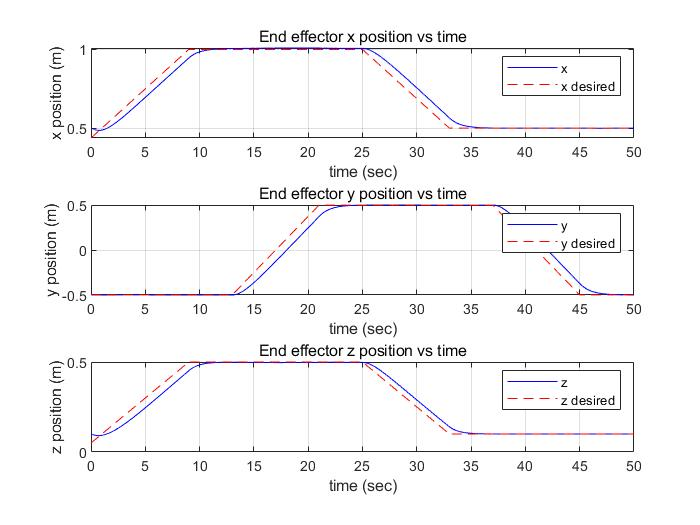
\includegraphics[width=8cm]{./fig/5.jpg}
	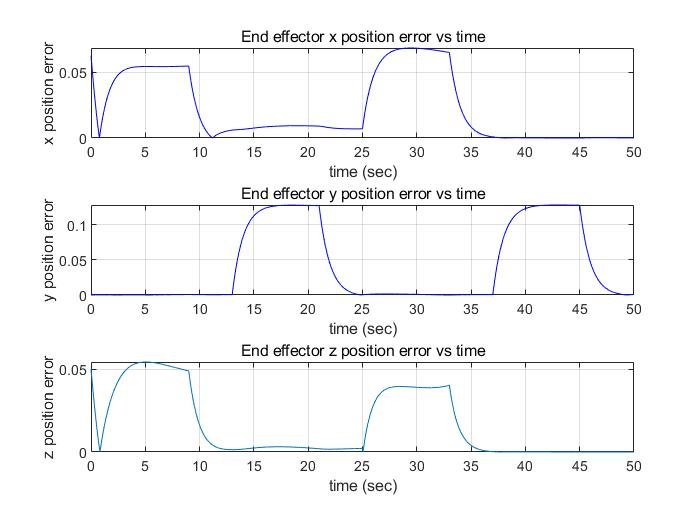
\includegraphics[width=8cm]{./fig/6.jpg}
	\caption{End Effector Position vs Time}
	\label{F 5.12}
\end{figure}

\newpage
\section{Conclusion}

In conclusion, we successfully built the four-arm robot and achieve the function of welding in a specific area. We designed all the relevant data and reduced the errors by simulink. The maximum error in end effector position on the x and z axes is below 0.05, while the maximum error on the y axis is slightly over 0.10, and the largest error of joint angle is joint2 angle, and it just nearly reaches 0.02. These errors are far better than the standards set. Overall, we achieved the desired results. This is certainly a product worth buying and will bring unimaginable benefits to your company.

%\section*{List of Symbols}
\begin{table}[H]
\centering
\begin{tabular}{lll}
 \toprule
  \textbf{Symbol}   &\textbf{Unit}      &\textbf{Explanation}\\
  \midrule
    n               & \si{\mole}        & Amount of substance \\
    m               & \si{\kilo\gram}   & Mass \\
    H               & \si{\kilo\joule\per\mole} & Molar enthalpy \\
    S               & \si{\joule\per\kelvin\per\mole}   & Molar entropy \\
    G               & \si{\kilo\joule\per\mole} & Gibbs free energy \\
    A               & \si{\kilo\joule\per\mole} & Helmholtz free energy \\
  \bottomrule
  \end{tabular}
\end{table}

%%%%%%%%%%%%%%%%%%%%%%%%%%%%%%%%%%%%%%%%%%%%%%%%%%%%%%%%%%
% Bibliography
%\newpage
\bibliographystyle{IEEEtran}
\bibliography{mendeley.bib}
%%%%%%%%%%%%%%%%%%%%%%%%%%%%%%%%%%%%%%%%%%%%%%%%%%%%%%%%%%
% Appendix
%\appendix
%\pagenumbering{roman}
%\section{First Appendix}
\label{app:first_appendix}
%\section{Second Appendix}
%\section{Third Appendix}
\end{document}
